\chapter{Grundlagen}
\label{ch:grundlagen}
Das folgende Kapitel beschreibt elementare Grundlagen, die zum Verständnis der nachfolgenden Kapitel notwendig sind. Der
erste Abschnitt befasst sich mit den verwendeten Maschinen und Komponenten der Robert Bosch Packaging GmbH.

Der zweite Teil widmet sich der Künstlichen Intelligenz und den verschiedenen Untergruppen und Ausprägungen, welche in
diesem Bereich existieren. Es wird dabei unter anderem auf die Konfiguration der Produkte und Laufzeitumgebungen
eingegangen. Außerdem werden hier die Programme und Konzepzte behandelt, welche in dieser Arbeit benötigt werden.

Im letzten Teil des Kapitels folgt die Beschreibung einer Designidee bei Smartphone-Apps, allgemeine Konzepte der
Softwareentwicklung und ein Framework zum Entwickeln von Webseiten.

\section{Bosch KWE Waage}
Die KWE Serie ist ein modulares Kontrollwaagensystem, das speziell für den Einsatz in der pharmazeutischen
Produktion entwickelt wurde.Dabei wurde sowohl besonderer Wert auf pharmazeutische Sicherheit und die Einhaltung der
GMP-Vorschriften gelegt, als auch auf die einfache Bedienung und die Flexibilität.

Die KWE 4000 kann bei einer maximalen Ausbringungsleistung von bis zu 450 P/min eine Genauigkeit ab 50mg erreichen.
Produktionsstatistiken, Trendkurven und das aktuelle Gewicht werden auf dem Standdarddisplay angezeigt.Durch individuelle
Konfigurationsmöglichkeiten, können je nach Bedarf auch weitere Informationen angezeigt werden.

Weitere Informationen auf der Übersichtsseite des Herstellers~\cite{online_grundlagen_boschkwe}.

\begin{figure}[h]
    \centering
    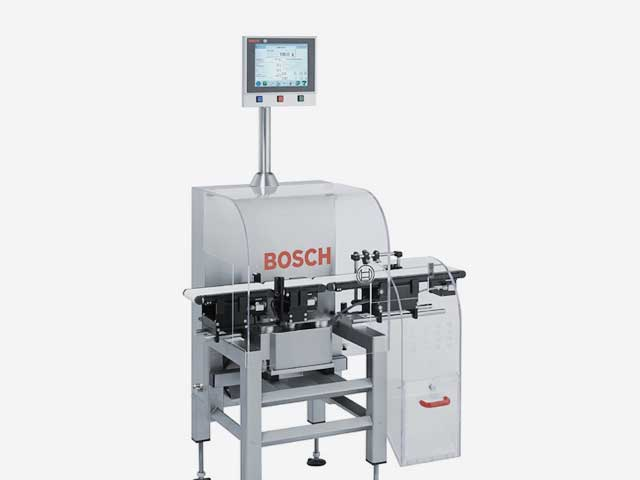
\includegraphics[scale=0.3]{images/kapitel_2/bosch_kwe.jpg}
    \caption{Abbildung einer Bosch KWE 3000}
    \label{fig:grundlagen_boschkwe}
\end{figure}

\section{Künstliche Intelligenz}
Was ist künstliche Intelligenz?

\colorbox{yellow}{Hier fehlt was}

In Abbildung~\ref{fig:grundlagen_artificialintelligence} auf Seite~\pageref{fig:grundlagen_artificialintelligence} ist
die Einordnung der Künstlichen Intelligenz in ihre Untergruppen ersichtlich. Dabei handelt es sich um eine eigene
Darstellung frei nach CodesOfInterest\footnote{https://codesofinterest.com/2016/11/difference-artificial-intelligence-machine-learning-deep-learning.html}.

\begin{figure}[h]
    \centering
    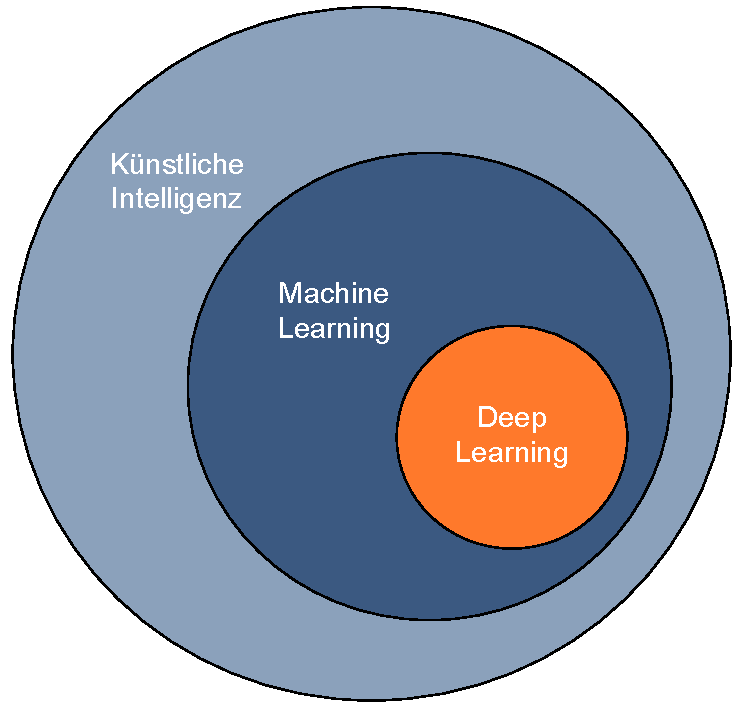
\includegraphics[scale=0.6]{images/kapitel_2/kuenstliche_intelligenz.pdf}
    \caption{Unterscheidung der Künstlichen Intelligenz}
    \label{fig:grundlagen_artificialintelligence}
\end{figure}

\section{Machine Learning}
Was ist Machine Learning?
\colorbox{yellow}{Hier fehlt was}

\subsection{Algorithmen}
Welche Algorithmen gibt es dafür
\colorbox{yellow}{Hier fehlt was}

\subsection{Bewertungskriterien}
Welche Bewertungskreterien gibt es
\colorbox{yellow}{Hier fehlt was}

\subsection{Klassifikation}
Welche Klassifikationen gibt es
\colorbox{yellow}{Hier fehlt was}

\subsection{Deep Learning}
Was ist Deep Learning
\colorbox{yellow}{Hier fehlt was}

\subsection{Neuronale Netze}
Was ist ein Neuronales Netz
\colorbox{yellow}{Hier fehlt was}

\section{Cloud}
Der Begriff Cloud hat sich als Kurzform des Cloud Computing etabliert und versteht das Zusammenspiel von mehreren Servern.
Die Server übernehmen Aufgaben, wie etwa die Datenspeicherung oder komplizierte Programmabläufe. Dabei erkennt der
Cloud-Nutzer nicht, wie viele Server hinter der Cloud stecken oder wo diese sich befinden.

Selbst wenn ein Server ausfällt, hat dies keine Auswirkungen auf das gesamte System, da die Anfragen und Aufgaben auf
die anderen Systeme umgeleitet werden.

Die Cloud zeichnet sich nach NIST~\cite{online_grundlagen_cloud_nist} und~\cite{online_grundlagen_cloud_computing} durch
fünf wesentliche Eigenschaften aus:

\begin{itemize}
    \item \textbf{On-Demand Self Service} \\
    Registrierte Nutzer können Resourcen selbstständig instantiieren und konfigurieren.
    \item \textbf{Broad Network Access} \\
    Der Zugriff kann von verschiedenen Endgeräten erfolgen.
    \item \textbf{Resource Pooling} \\
    Alle Resourcen des Anbieters werden gebündelt und nach Bedarf den Nutzern zugewiesen.
    \item \textbf{Rapid Elasticity} \\
    Kapazitäten können nach Bedarf skaliert werden und stehen schnell und dynamisch zur Verfügung.
    \item \textbf{Measured Service} \\
    Es existiert eine automatische Kontrolle der Ressourcen durch einen Zähler, welcher die Transparenz für den
    Anbieter und den Benutzer ermöglicht.
\end{itemize}

Auf dem Markt existieren zahlreiche Cloud-Anbieter. Im folgenden wird auf drei der Top 10 größten Anbieter und deren
Lösungen im Bereich künstliche Intelligenz eingegangen (siehe hierzu~\cite{online_grundlagen_cloud}).

\subsection{Microsoft Azure}
Die Cloud-Computing-Plattform Azure von Microsoft ist hoch skalierbar und wendet sich mit ihren Services hauptsächlich
an Unternehmen und Entwickler. Verfügbar ist Azure offiziell seit dem Jahr 2010. Seither erweitert Microsoft das
Serviceangebot und die Leistungsfähigkeit seiner Cloud-Computing-Umgebung kontinuierlich.

User können Services aus den Bereichen Infrastructure as a Service (IaaS), Platform as a Service (PaaS) und Software as
a Service (SaaS) aus der Cloud beziehen. Auch Datenbanken und Storagesysteme werden bereitgestellt. Ziel ist es,
Anwendern eine flexible Cloud-Infrastruktur zur Verfügung zu stellen, die sich den individuellen Anforderungen schnell
anpassen lässt und den Betrieb einer eigenen IT-Infrastruktur überflüssig macht. Zahlreiche Standarddienste wie virtuelle
Maschinen, SQL-Datenbanken oder VPN-Gateways können genutzt werden.

Dank professionell betriebener Rechenzentren in der ganzen Welt stehen die Dienste mit einer hohe Verfügbarkeit überall
zur Verfügung. Microsoft Azure ermöglicht den Einsatz von Hybrid-Systemen, bei denen nur ein Teil der Services,
Anwendungen und Daten in die Cloud verlagert sind und der Rest auf lokalen Servern betrieben wird. Dienste von
Drittanbietern bietet ein eigener Azure Marktplatz an (mehr unter~\cite{online_grundlagen_azure}).

\subsubsection{Azure Machine Learning Studio}
Microsoft Azure Machine Learning Studio ist ein Tool für die Zusammenarbeit per Drag \& Drop, mit der Sie Lösungen für
Vorhersageanalysen erstellen, testen und bereitstellen können, die mit Ihren Daten arbeiten. Machine Learning Studio
veröffentlicht Modelle als Webdienste, die von benutzerdefinierten Apps oder BI-Tools wie Excel problemlos genutzt werden
können (siehe dazu~\cite{article_grundlagen_azure_studio}).

In Machine Learning Studio finden Datenwissenschaften, prädiktive Analysen, Cloudressourcen und Ihre Daten zusammen!

\subsection{Amazon Web Services}
AWS, eine Tochterfirma von Amazon.com, ist eine umfangreiche Plattform für Cloud Computing Services. Cloud Computing
beinhaltet in der Regel die drei Bestandteile Infrastucture as a Service (IaaS), Platform as a Service (PaaS) und
Software as a Service (SaaS).

IaaS bedeutet, dass Kunden über das Internet Zugang zu den verfügbaren IT-Services haben, beispielsweise im Bereich
Datenspeicherung oder Rechenleistung, und diese überall und an verschiedenen Endgeräten nutzen können. Der Begriff PaaS
beschreibt die Nutzung einer Cloud-Plattform zur Entwicklung von Webanwendungen. SaaS steht für die Bereitstellung
browserbasierter Software durch einen externen Dienstleister, die von mehreren Usern gleichzeitig genutzt werden kann.
Ein bekanntes Beispiel hierfür ist Google Docs, das eine standortunabhängige Bearbeitung von Dokumenten ermöglicht.

Für Unternehmen sind Public Clouds beispielsweise nützlich, um schnell und einfach individuelle Anwendungen entwickeln
zu können, ohne eigene Produktlizenzen oder Serverplätze erwerben zu müssen. Oder anders gesagt: AWS stellt Entwicklern
eine maßgeschneiderte und zuverlässige IT-Infrastruktur auf Abruf zur Verfügung (= Self Service)
(mehr unter~\cite{online_grundlagen_aws}).

\subsubsection{Amazon Machine Learning}
Amazon Machine Learning ist ein Service, mit dem Entwickler aller Wissensstufen die Technologie für machinelles Lernen
problemlos nutzen können. Amazon Machine Learning bietet Visualisierungstools und Assistenten, die Sie durch den
Aufbauprozess für Machine Learning-Modelle (ML) begleiten, ohne dass Sie komplexe ML-Algorithmen und ‑Technologien
erlernen müssen. Wenn Ihre Modelle fertig sind, können Sie bei Amazon Machine Learning mithilfe einfacher APIs Prognosen
für Ihre Anwendung abrufen, ohne benutzerdefinierte Prognosecodes implementieren oder Infrastrukturen verwalten zu müssen.

Amazon Machine Learning basiert auf der gleichen praxisbewährten, hochgradig skalierbaren ML-Technologie, die seit Jahren
von der internen Community der Amazon-Datenwissenschaftler verwendet wird. Der Service nutzt leistungsstarke Algorithmen,
um ML-Modelle zu erstellen, indem er in Ihren vorhandenen Daten nach Mustern sucht. Anschließend verwendet Amazon Machine
Learning diese Modelle, um neue Daten zu verarbeiten und Prognosen für Ihre Anwendung zu generieren.

Amazon Machine Learning ist hochgradig skalierbar und kann Milliarden von Prognosen pro Tag generieren und diese in
Echtzeit mit hohem Durchsatz bereitstellen. Für die Nutzung von Amazon Machine Learning sind keine Vorab-Investitionen
für Hardware oder Software erforderlich. Sie bezahlen für das, was Sie nutzen, können also klein beginnen und skalieren,
wenn Ihre Anwendung wächst (mehr dazu in der Dokumentation~\cite{online_grundlagen_aws_learning})

\subsection{IBM Cloud (ehemals Bluemix)}
Bluemix ist die von IBM entwickelte Cloud-Platform. Über Bluemix greifen Entwickler auf mehr als 160 Cloud-Services zu,
um mobile Apps und Webanwendungen zu entwickeln. In Bluemix gibt es zahlreiche Analysewerkzeuge sowie Services von
Drittanbietern. Mit Watson Analytics lassen sich beispielsweise intelligente Systeme realisieren, die Daten kognitiv
(also selbstlernend, ohne für die Problemlösungen programmiert zu sein) auswerten und für die Entscheidungsfindung
aufbereiten.

Bluemix unterstützt diverse integrierte DevOps-Dienste, um Cloud-Anwendungen zu erstellen, auszuführen, bereitzustellen
und zu verwalten. Die Entwicklerplattform basiert auf der Technologie von Cloud Foundry und läuft auf IBMs
Softlayer Cloud Infrastruktur. Sie unterstützt mehrere Programmiersprachen, einschließlich Java, Node.js, Go, PHP,
Python, Ruby Sinatra, Ruby on Rails und kann auch andere Sprachen wie Scala durch den Einsatz von Buildpacks
unterstützen~\cite{book_grundlagen_bluemix}.

Weitere Informationen üer Bluemix können auf der Webseite\footnote{https://bluemix.net} gefunden werden.

\subsubsection{Watson Studio}
Watson Studio is an integrated environment designed to make it easy to develop, train, manage models and deploy
AI-powered applications. It is a SaaS solution delivered on the IBM Cloud.

Watson Studio provides a suite of tools for data scientists, application developers and subject matter experts to
collaboratively and easily work with data. They can then use that data to build, train and deploy models at scale. These
tools are preconfigured, so builders don't have to spend time installing, setting up and maintaining them. The built-in
catalog function enables knowledge sharing and retention. Watson Studio can infuse AI into your business
(mehr hierzu unter~\cite{online_grundlagen_watson_studio}).

\subsubsection{Cloud Object Storage}
Cloud object storage is a format for storing unstructured data in the cloud. Object storage is considered a good fit for
the cloud because it is elastic, flexible and it can more easily scale into multiple petabytes to support unlimited data
growth. The architecture stores and manages data as objects compared to block storage, which handles data as blocks, and
logical volumes and file storage which store data in hierarchical files.


The object storage software design includes a globally unique identifier for each object along with rich, customizable
metadata. The metadata is separated to enable other capabilities such as application- and user-specific data for
indexing, interfaces that can be directly programmed by the application, a global namespace and more flexible data
management policies (mehr dazu unter~\cite{book_grundlagen_objectstorage}).

\subsubsection{Apache Spark}
Bei Apache Spark handelt es sich um ein Framework, das unter Open-Source-Lizenz öffentlich verfügbar ist. Es ist ein Top
Level Project der Apache Software Foundation und entstand ursprünglich aus einem Forschungsprojekt an der University of
California in Berkeley.

Spark ermöglicht es, Datenabfragen auf große Datenmengen aus unterschiedlichen Quellen in hoher Geschwindigkeit und
guter Performance auszuführen. Hierfür nutzt das Framework eine verteilte Architektur und Cluster Computing. Viele
große Unternehmen unterstützen die Apache Software Foundation und treiben die Entwicklung von Spark weiter voran
(mehr dazu unter~\cite{book_grundlagen_apachespark}).

\subsubsection{API Connect}
IBM API Connect richtet sich an Unternehmen, die ihren Weg in die API-Economy optimieren und beschleunigen wollen.
Diese umfassende Managementlösung deckt alle vier Aspekte des API-Lebenszyklus ab: Erstellung, Ausführung, Management
und Schutz. API Connect ist sehr viel kosteneffizienter als Einzellösungen, die sich nur auf wenige Phasen des
Lebenszyklus beschränken. Mit API Connect können externe und interne Nutzer das API-Programm eines Unternehmens
beschleunigen und neuen Umsatz durch attraktive neue Kundenerlebnisse schaffen
(mehr in der Dokumentation~\cite{book_grundlagen_apiconnect}).

\subsubsection{Toolchain}
Bei einer Toolchain handelt es sich um ein Tool zur Verwaltung von Entwicklung, Bereitstellung sowie Üerwachung einer
Anwendung. Nach der Einrichtung einer Toolchain stehen verschiedene Services zur Verfügung, welche zum Beispiel eine
Integration zu einem GitHub-Projekt ermöglichen.

Mit einer eingerichteten Toolchain und einem verbundenen Git-Repository kann der Quelltext gebaut und auf einem System
installiert werden. Bei der Toolchain handelt es sich unter anderem um ein \textit{Continuous Integration}-Tool (kurz CI)
(Mehr unter~\cite{online_grundlagen_toolchain}).

\section{TensorFlow.js}
Tensorflow ist eine Deep Learning Bibliothek welches von Google entwickelt wird und unter der freien Apache 2.0 Open
Source Lizenz zur Verfügung gestellt. Durch die Repräsentation von Neuronalen Netzwerken in Graphen können diese auf
verteilte Computersysteme abgebildet werden. Zum Einsatz kommt es in verschiedenen Projekten von Google, wie Google
Translate und DeepMind und hilft dort z.B. bei der Erkennung von Objekten auf Fotos und Videos. Weiterhin wird es
beispielsweise für Predictive Analytics, Fraud Detection aber auch als Recommendation Engine verwendet.

Tensorflow ist der Nachfolger von Googles erstem Deep Learning Tool DistBelief, das aus Google Brain, einem Deep
Learning Forschungs-Projekt, hervor ging. Es wurde in verschiedenen internen Projekten von diversen Teams benutzt.
Allerdings hatte „DistBelief“ einige Fehler im Aufbau und Design, die das Tool unflexibel und schlecht nutzbar machten.
Mit dem Wissen über diese Fehler wurde das Projekt Tensorflow gestartet und im November 2015 zum ersten Mal vorgestellt.
Aufgrund der einfachen Handhabung und den vielfältigen Möglichkeiten wurde es schnell in vielen Machine Learning
Projekten eingesetzt. Beispielsweise bei Natural Language Processing, künstlicher Intelligenz und Predictive Analytics.

Für Data Science und Machine Learning Experten stellt es eine geeignete Basis dar, mit dem performante Machine Learning
Lösungen bereitgestellt werden. In der neuesten Version lässt sich Tensorflow ohne großen Aufwand in Python integrieren,
dadurch können neue Lösungen einfach zur Verfügung gestellt werden (mehr unter~\cite{book_grundlagen_tensorflow}).

\section{Angular}
Angular ist ein JavaScript-Framework welches von Google entwickelt wurde. Es zielt auf die Entwicklung von
WebAnwendungen legt großen Wert auf Struktur und Qualität. Es war das erste Framework welches durch den Fokus auf
Architektur, Testing und isolierte Komponenten im JavaScript-Bereich auch für große Enterprise Anwendungen geeignet war.
Durch Methoden wie Dependency Injection und ein ausgereiftes Tooling ermöglicht es effiziente und wartbare
Softwareentwicklung auf Basis von JavaScript (mehr unter~\cite{book_grundlagen_angular}).

\subsection{Model-View-Controller}
Model-View-Controller (kurz MVC) wurde um 1978 von Xerox entwickelt und es handelt sich dabei um eine Architektur von
Programmen.

In MVC wird eine Anwendungskomponente in drei Teile zerlegt. In das oberflächenunabhängige \textit{Model}, das für die
Ausgabe zuständige \textit{View} und den für die Interpretation von Eingabeereignissen zuständigen \textit{Controller}.

Der Controller ist die Steuerungseinheit, das Model der Anwendungskern und die View der Darsteller bzw. die Ansicht der
Anwendung. Ein View zusammen mit seinem Controller wird hier auch als eine Oberfläche bezeichnet (Mehr hierzu
unter~\cite{book_grundlagen_mvc}).

Es gibt zahlreiche Frameworks, welche das MVC-Patern umsetzen. Angular ist einer der bekanntesten Vertreter.

\subsection{Angular-Material}
Material Design ist eine von Google stetig weiterentwickelte Designsprache. Sie verbindet die Gestaltungsregeln des
klassischen Grafik-Designs mit den Möglichkeiten digitaler Benutzeroberflächen. Ziel von Material Design ist u.a. die
Verbesserung der Benutzerfreundlichkeit. Darüber hinaus hat Material Design einen charakteristischen Look, so dass im
Material Design gestaltete Interfaces sich ideal kombinieren lassen (mehr dazu~\cite{online_grundlagen_materialdesign}).

Mittels der Library \textit{Angular-Material} kann das Material Design in einer Angular Applikation leicht umgesetzt
werden.

\subsection{ngx-restangular}
Ngx-restangular is an Angular 2+ service that simplifies common GET, POST, DELETE, and UPDATE requests with a minimum of
client code. It's a perfect fit for any WebApp that consumes data from a RESTful API
(mehr auf deer betreffenden GitHub-Seite~\cite{online_grundlagen_restangular}).

\subsection{Observable}
Ein Observable ist das zentrale Konzept in Reactive Programming mit ReactiveX (http://reactivex.io/). Ein Observable
repräsentiert eine Menge von Daten, die in einer noch nicht bekannten Menge zu einem noch nicht bekannten Zeitpunkt
bereitstehen werden. Ein Observer abonniert ein Observable und damit die später ankommenden Daten. Ein Obserable kann
gefiltert, gruppiert oder transformiert werden. Berechnungen sind möglich (mehr unter~\cite{book_grundlagen_observable}).

\subsection{Promise}
Um Promises verständlich zu machen, fangen wir mit einer groben Umschreibung an und gehen dann auf Details und konkrete
Anwendungen ein. Wenn ihr euch zunächst unter dem Begriff Promise nichts vorstellen könnt, seid ihr nicht allein.
Promises sind so etwas wie Callbacks 2.0. Diese Umschreibung trifft auch schon genau den Grund, warum ihr Promises nutzen
solltet. Dazu machen wir kurz noch einen Ausflug und frischen unser Wissen über Callbacks auf
(mehr in~\cite{book_grundlagen_promises}).

\subsection{flex-layout}
Angular Flex Layout provides a sophisticated layout API using Flexbox CSS + mediaQuery. This module provides Angular
developers with component layout features using a custom Layout API, mediaQuery observables, and injected DOM
flexbox-2016 CSS stylings.

The Flex Layout engine intelligently automates the process of applying appropriate Flexbox CSS to browser view
hierarchies. This automation also addresses many of the complexities and workarounds encountered with the traditional,
manual, CSS-only application of box CSS (mehr auf der GitHub-Pages~\cite{online_grundlagen_flexlayout}).

\section{REST}
REST-API steht für Representational State Transfer - Application Programming Interface. Diese Interfaces machen den
Austausch von Informationen uüber unterschiedliche Systeme möglich. Im Zeitalter verteilter Systeme und Cloud-Computing
trifft man oft auf unterschiedliche Systeme, welche den Einsatz von REST-API notwendig machen.

Man spricht bei REST-API auch von der Maschine-Maschine-Kommunikation, da die verschiedenen Systeme und Geräte
zusammengebracht werden und gewissermaßen die gleiche Sprache sprechen.

Mit REST-API ist es möglich geworden, Informationen und Aufgaben auf verschiedene Systeme zu verteilen und diese mit der
Hilfe von HTTP-Requests anzufordern. Jeder HTTP-Request setzt sich aus dem Endpoint und den entsprechenden Parametern
zusammen~\cite{online_grundlagen_rest}.

\section{Cloud Foundry}
Cloud Foundry ist eine Open Source Platform as a Service (PaaS) Lösung. Mit Hilfe von Cloud Foundry können Entwickler
ihre Anwendungen bauen, hochladen und ausführen. Ein großer Vorteil von Cloud Foundry ist die nahezu grenzenlose
Skalierbarkeit~\cite{book_grundlagen_cloudfoundry}.

Die Skalierbarkeit wird durch die Container-Architektur erreicht. Jeder Container beinhaltet eine eigene Anwendungsinstanz.
Dabei wird sowohl eine horizontale als auch eine vertikale Skalierung unterstützt.

Bei der horizontalen Skalierung werden zusätzliche Container gestartet oder gestoppt und ein Load Balancer vor die
Container geschaltet. Bei der vertikalen Skalierung werden jeder Instanz individuell z.B. mehr oder weniger Arbeitsspeicher
zugeteilt.

Jede Cloud Foundry Instanz besitzt eine IPV4-Adresse wodurch es mittels A-Record (Zuordnung eines DNS-Namens zu IP-Adresse)
möglich ist, eine eigene Domain mit der Anwendung zu verknüpfen.

\section{Version Control (Git)}
Git ist ein verteiltes Versionierungssystem welches frei als Open-Source zur Verfügung gestellt wird. Einige bekannte
Namen wie der Linux-Kernel, Eclipse oder Android verwenden Git für die Verwaltung ihrer Projekte.[1] Ähnlich zu
Subversion (SVN) wird Git für die Versionskontrolle (stetige Protokollierung von Änderungen) von Dateien eingesetzt. Im
Gegensatz zu SVN gibt es jedoch einige grundlegende Unterschiede, andere Begriffe und Schemata können aber auch direkt
umgelegt werden (mehr unter~\cite{book_grundlagen_git}).

\section{Node Package Manager (npm)}
Unter NPM (Node Package Manager) versteht man ein Paketmanager für node.js. Mit NPM lassen sich unter anderem
Software-Pakete für die Entwicklung von Webprojekten verwalten und steuern. Mehrere tausend OpenSource-Pakete lassen sich
unter dem Namen npm Registry bzw. npm Open Source finden und verwenden (mehr unter~\cite{book_grundlagen_npm}).

\section{Mockups}
Ein Mockup kommt während der Planung eines Webauftritts zum Einsatz. Mit der Hilfe eines Mockups kannst du deine neue
Website sehr schnell und einfach visualisieren und erhälst einen ersten Eindruck von der Gestaltung und den
Funktionalitäten deiner Website. Dazu brauchst du nicht eine Zeile Quellcode schreiben, da Mockups entweder auf Papier
entworfen oder über sogenannte Mockup-Tools am PC realisiert werden.

Bei einem Mockup tritt das Design der Website in den Hintergrund. Hier geht es einzig und alleine darum, die
verschiedenen Elemente deiner Website anzuordnen und somit einen optimalen Userflow zu realisieren. Im Fokus steht
dabei die Planung der Interaktionsmöglichkeiten und Funktionen deiner Website (mehr unter~\cite{book_grundlagen_mockups}).

\section{TypeScript}
TypeScript (kurz: TS) ist ein Superset von JavaScript. Das bedeutet, TS ist ebenfalls eine Implementierung von ECMAScript,
erweitert aber JavaScript mit zusätzlichen Features. Jeder JavaScript-Code funktioniert auch in TypeScript, aber nicht
jeder TypeScript-Code funktioniert auch in JavaScript.

Wie der Name schon verrät, erweitert TypeScript JavaScript um Typings (und Annotations). Das heißt die Programmiersprache
ist Typsicher. Wie z.B. auch Java (mehr unter~\cite{book_grundlagen_typescript}).

\begin{lstlisting}[language=JavaScript, caption=Unterschied zwischen JavaScript und TypeScript, label=Unterschied zwischen JavaScript und TypeScript]
    // JavaScript
    var name = "Vorname Nachname";

    // TypeScript
    let name : string = "Vorname Nachname";
\end{lstlisting}

\section{WebView}
Bei WebView handelt es sich um ein Android- und iOS-Layout, das Webseiten darstellen kann. Über Schnitstellen werden
Informationen wie Webseite, URL und Größe üergeben. Das Laden, das Anzeigen und die Interaktion mit der Webseite üernimmt
das Layout selbstständig.

Das Layout steht sowohl unter Android als auch iOS in den frühesten Versionen zur Verfügung (Weitere Informationen
unter~\cite{online_grundlagen_webview}).